% Editable native annotations around unchanged verified IDE photographs.
\par
\begin{figure}[htbp]
\centering
\newsavebox{\MARSwavpipelineregistersBox}
\sbox{\MARSwavpipelineregistersBox}{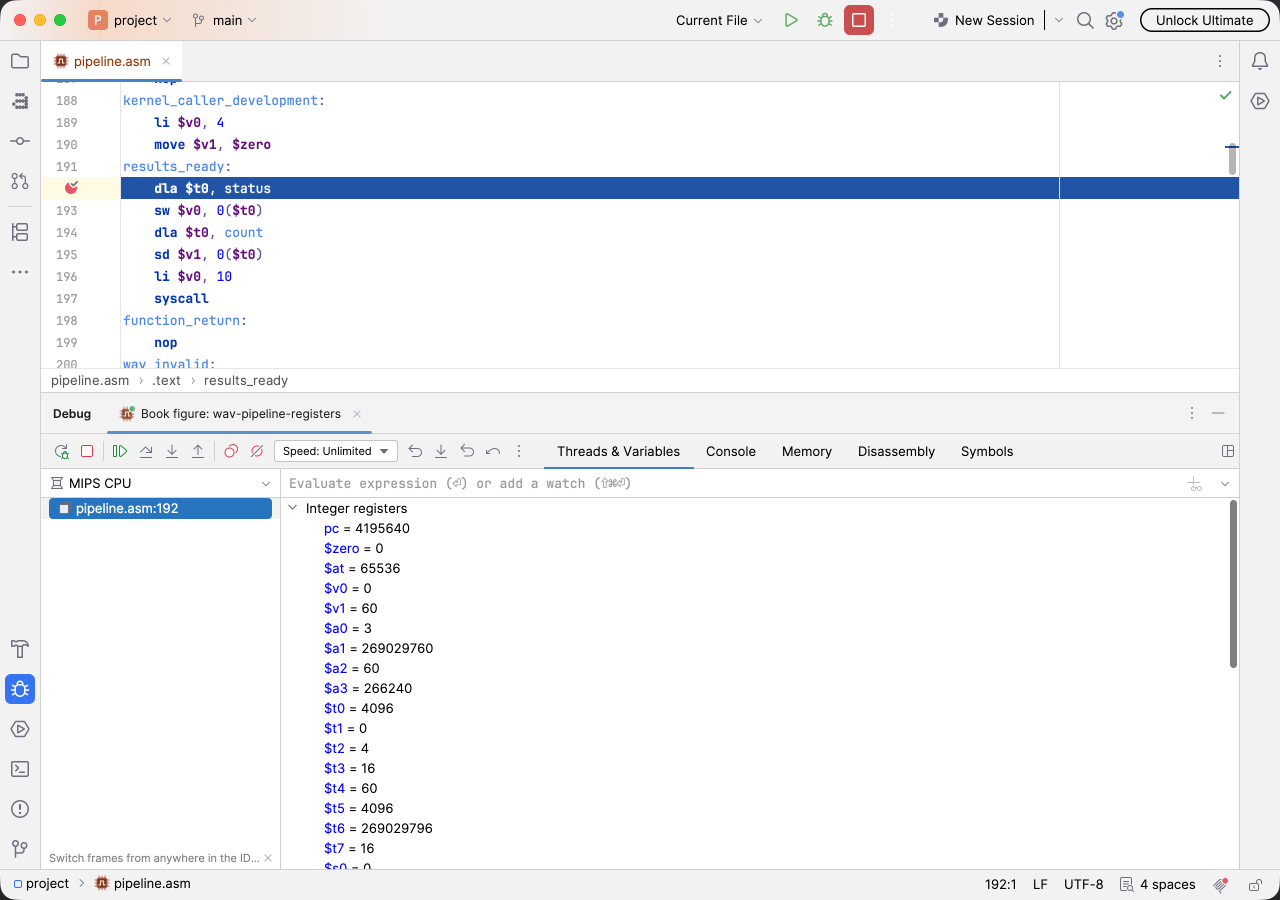
\includegraphics[artifact]{packages/031-pcm-wav/captures/f05/registers.png}}
\newsavebox{\MARSwavpipelinesourceBox}
\sbox{\MARSwavpipelinesourceBox}{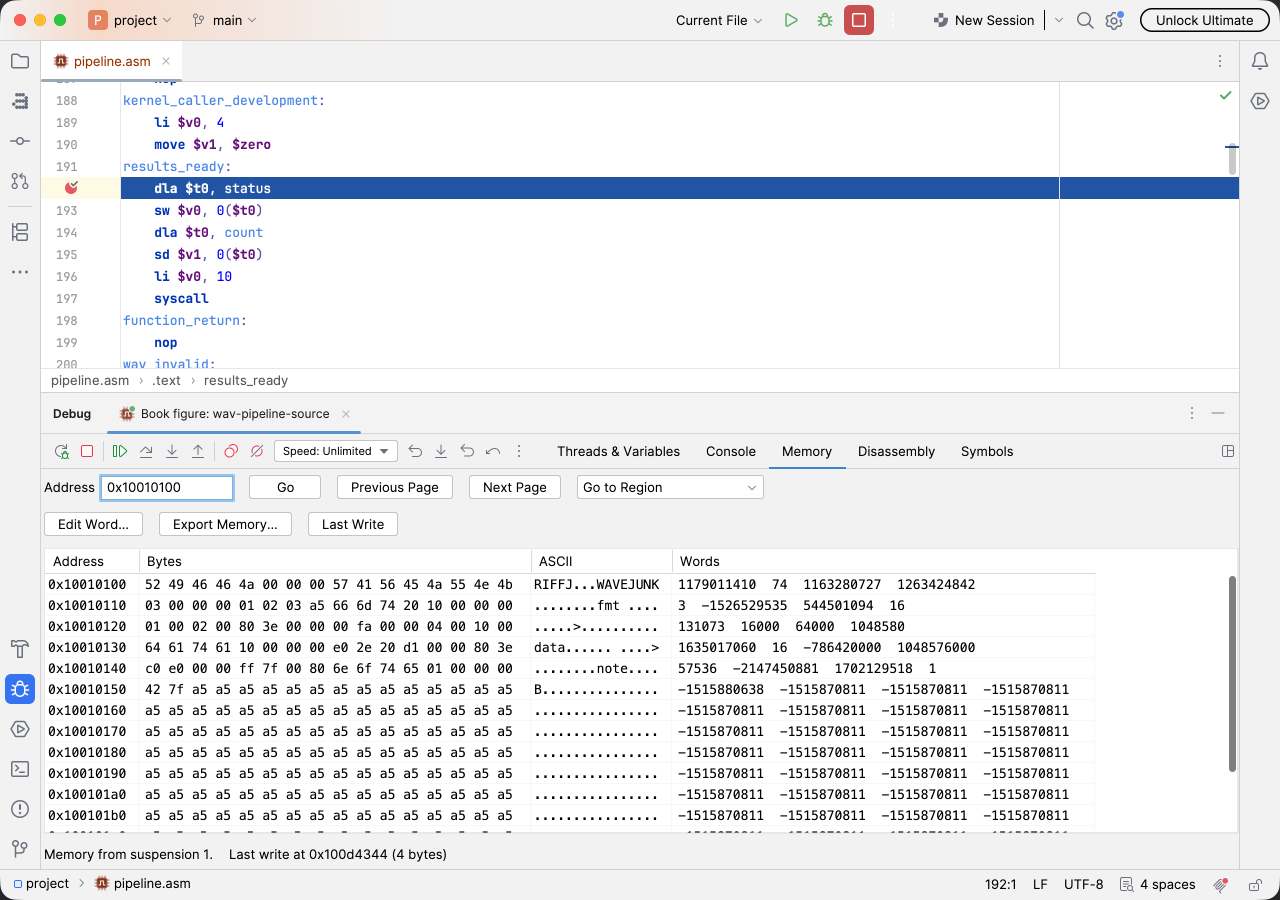
\includegraphics[artifact]{packages/031-pcm-wav/captures/f05/source.png}}
\newsavebox{\MARSwavpipelinedestinationBox}
\sbox{\MARSwavpipelinedestinationBox}{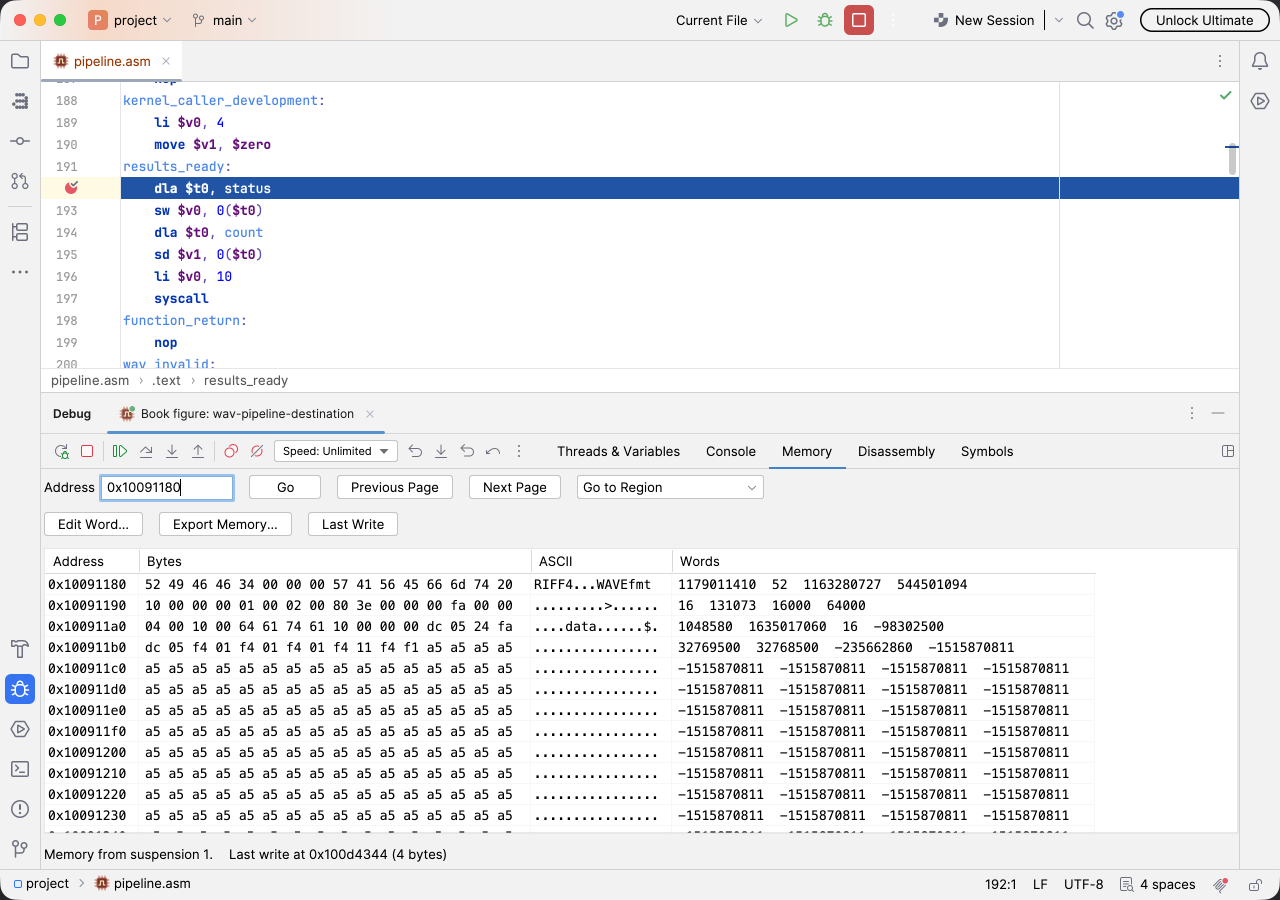
\includegraphics[artifact]{packages/031-pcm-wav/captures/f05/destination.png}}
\newsavebox{\MARSwavpipelineclipsBox}
\sbox{\MARSwavpipelineclipsBox}{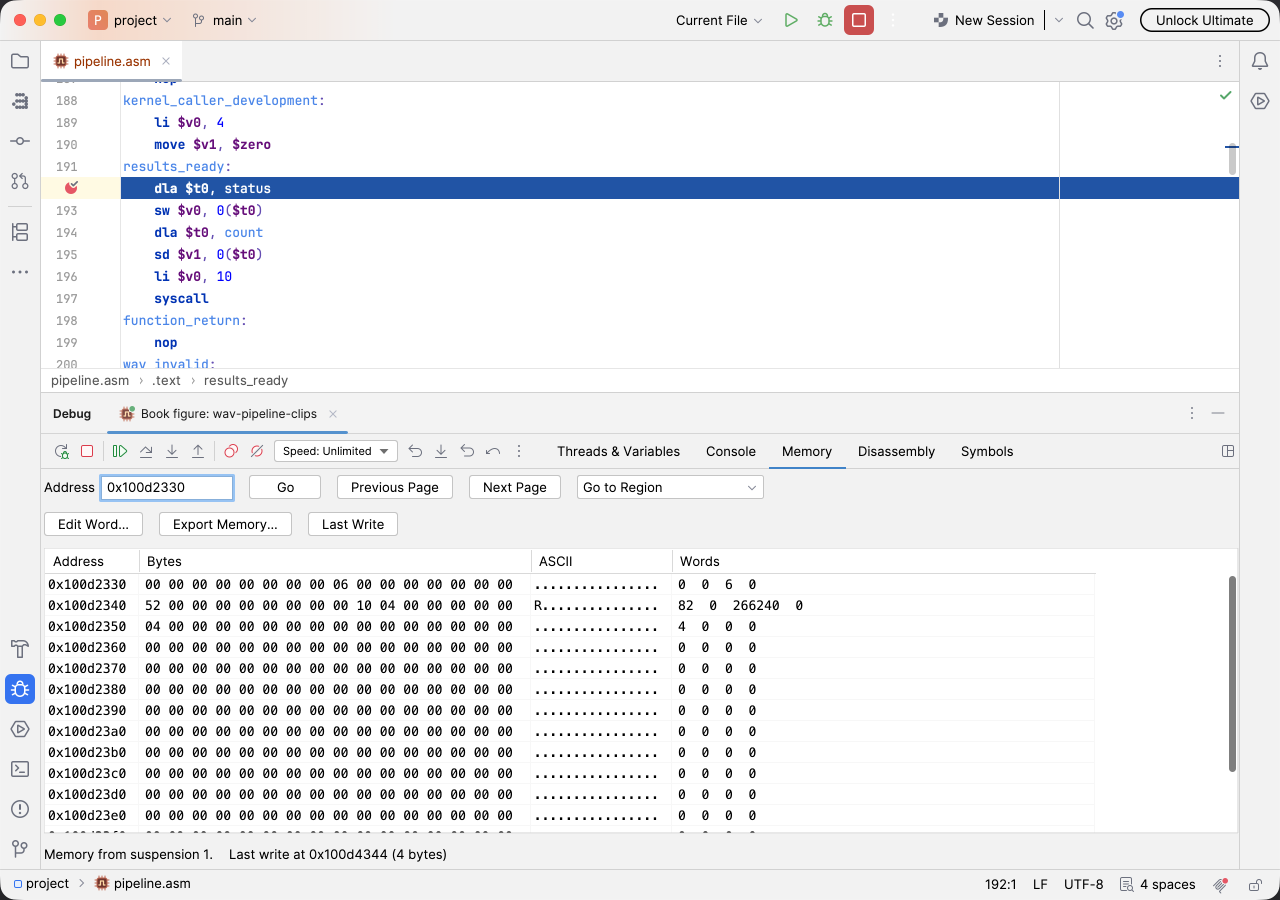
\includegraphics[artifact]{packages/031-pcm-wav/captures/f05/clips.png}}
\edef\MARSwavpipelinesourceLeft{\the\dimexpr0.036718750\wd\MARSwavpipelineregistersBox\relax}
\edef\MARSwavpipelinesourceBottom{\the\dimexpr0.774444444\ht\MARSwavpipelineregistersBox\relax}
\edef\MARSwavpipelinesourceRight{\the\dimexpr0.713281250\wd\MARSwavpipelineregistersBox\relax}
\edef\MARSwavpipelinesourceTop{\the\dimexpr0.170000000\ht\MARSwavpipelineregistersBox\relax}
\edef\MARSwavpipelinereturnsLeft{\the\dimexpr0.246093750\wd\MARSwavpipelineregistersBox\relax}
\edef\MARSwavpipelinereturnsBottom{\the\dimexpr0.312222222\ht\MARSwavpipelineregistersBox\relax}
\edef\MARSwavpipelinereturnsRight{\the\dimexpr0.553906250\wd\MARSwavpipelineregistersBox\relax}
\edef\MARSwavpipelinereturnsTop{\the\dimexpr0.640000000\ht\MARSwavpipelineregistersBox\relax}
\edef\MARSwavpipelineinputLeft{\the\dimexpr0.034375000\wd\MARSwavpipelinesourceBox\relax}
\edef\MARSwavpipelineinputBottom{\the\dimexpr0.217777778\ht\MARSwavpipelinesourceBox\relax}
\edef\MARSwavpipelineinputRight{\the\dimexpr0.584375000\wd\MARSwavpipelinesourceBox\relax}
\edef\MARSwavpipelineinputTop{\the\dimexpr0.608888889\ht\MARSwavpipelinesourceBox\relax}
\edef\MARSwavpipelineoutputLeft{\the\dimexpr0.034375000\wd\MARSwavpipelinedestinationBox\relax}
\edef\MARSwavpipelineoutputBottom{\the\dimexpr0.264444444\ht\MARSwavpipelinedestinationBox\relax}
\edef\MARSwavpipelineoutputRight{\the\dimexpr0.584375000\wd\MARSwavpipelinedestinationBox\relax}
\edef\MARSwavpipelineoutputTop{\the\dimexpr0.608888889\ht\MARSwavpipelinedestinationBox\relax}
\edef\MARSwavpipelineclipsLeft{\the\dimexpr0.034375000\wd\MARSwavpipelineclipsBox\relax}
\edef\MARSwavpipelineclipsBottom{\the\dimexpr0.334444444\ht\MARSwavpipelineclipsBox\relax}
\edef\MARSwavpipelineclipsRight{\the\dimexpr0.584375000\wd\MARSwavpipelineclipsBox\relax}
\edef\MARSwavpipelineclipsTop{\the\dimexpr0.608888889\ht\MARSwavpipelineclipsBox\relax}
\begin{tikzpicture}[alt={Five details at results_ready show successful status, returned output length 60, the complete 82-byte source, canonical output with PCM offset 44, and a separate zero clip count.}]
\node[anchor=north west,inner sep=0,font=\small\bfseries] (source-title) at (6mm,0) {Caller instruction before saving results};
\node[anchor=north west,inner sep=0] (source) at ([yshift=-1mm]source-title.south west) {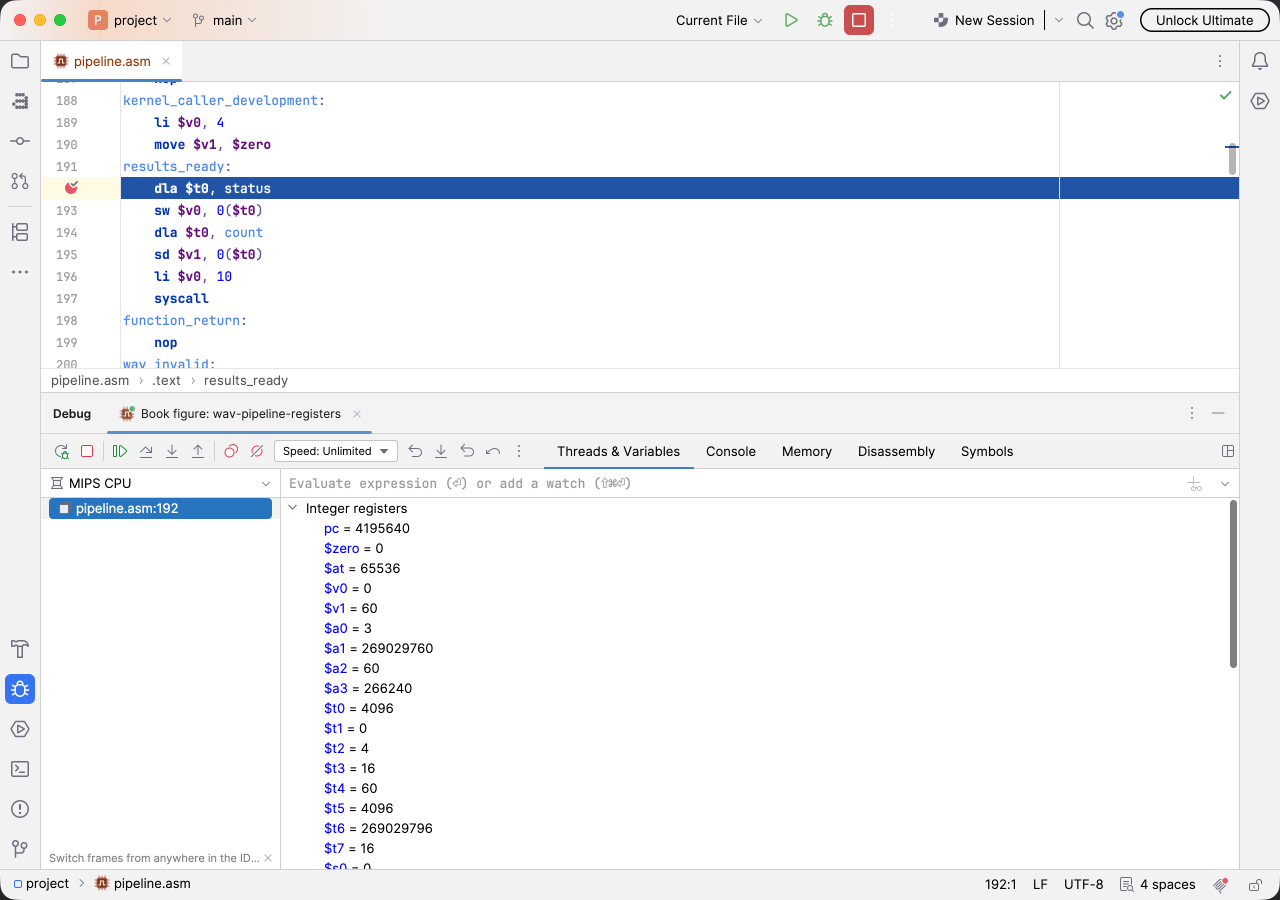
\includegraphics[width=0.52\linewidth,artifact,trim={\MARSwavpipelinesourceLeft{} \MARSwavpipelinesourceBottom{} \MARSwavpipelinesourceRight{} \MARSwavpipelinesourceTop{}},clip]{packages/031-pcm-wav/captures/f05/registers.png}};
\begin{scope}[shift={(source.south west)},x={($(source.south east)-(source.south west)$)},y={($(source.north west)-(source.south west)$)}]
\draw[black,line width=0.7pt] (0.237500000,0.080000000) rectangle (0.700000000,0.520000000);
\node[draw=black,fill=white,circle,inner sep=1.5pt,font=\footnotesize] at ($(0.237500000,0.520000000)+(-3mm,0)$) {1};
\end{scope}
\node[anchor=north west,inner sep=0,font=\small\bfseries] (returns-title) at (0.56\linewidth,0 |- source-title.north) {Success and canonical output length};
\node[anchor=north west,inner sep=0] (returns) at ([yshift=-1mm]returns-title.south west) {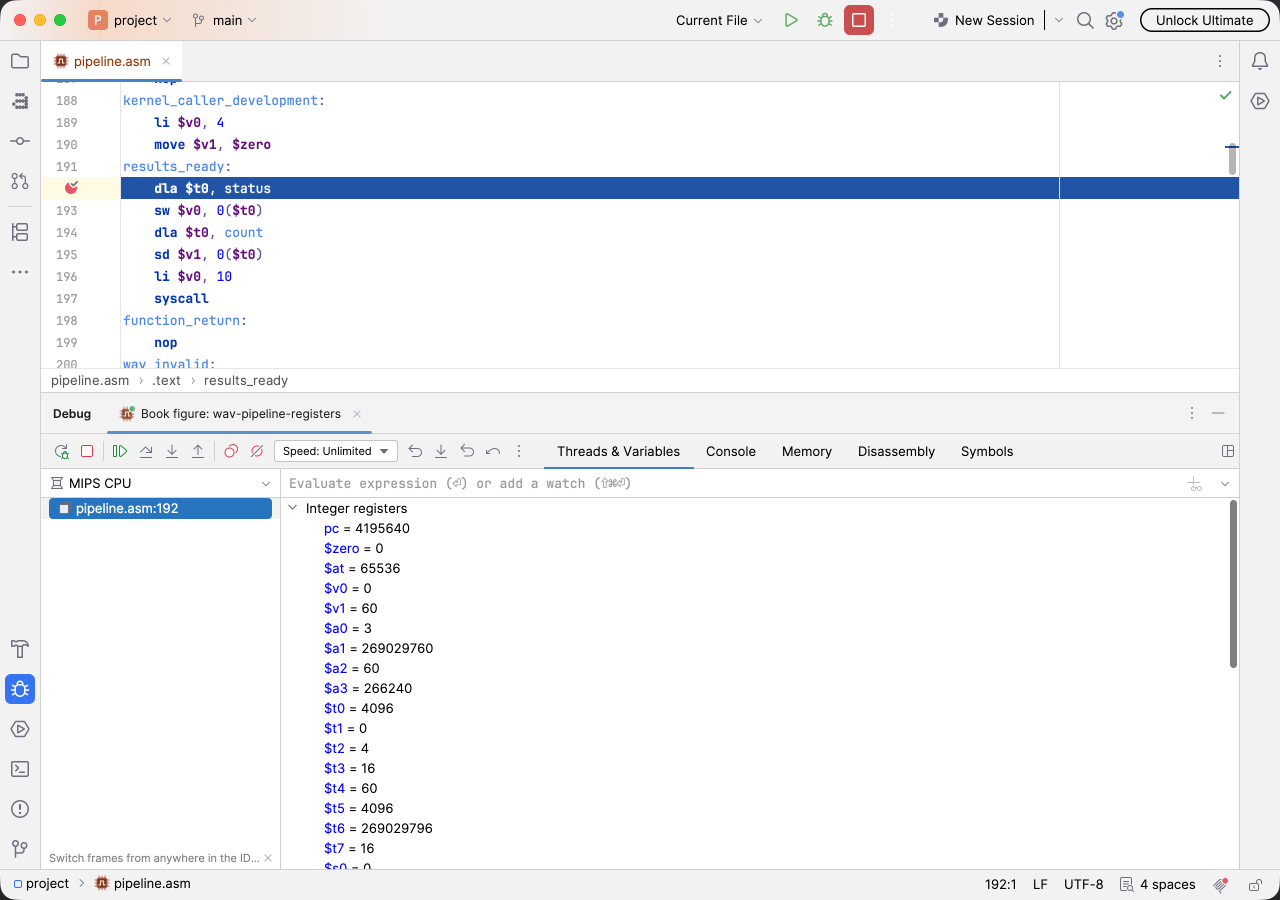
\includegraphics[width=0.44\linewidth,artifact,trim={\MARSwavpipelinereturnsLeft{} \MARSwavpipelinereturnsBottom{} \MARSwavpipelinereturnsRight{} \MARSwavpipelinereturnsTop{}},clip]{packages/031-pcm-wav/captures/f05/registers.png}};
\begin{scope}[shift={(returns.south west)},x={($(returns.south east)-(returns.south west)$)},y={($(returns.north west)-(returns.south west)$)}]
\draw[black,line width=0.7pt] (0.023437500,0.023255814) rectangle (0.250000000,0.953488372);
\node[draw=black,fill=white,circle,inner sep=1.5pt,font=\footnotesize] at ($(0.023437500,0.953488372)+(-3mm,0)$) {2};
\end{scope}
\node[anchor=north west,inner sep=0,font=\small\bfseries] (input-title) at ([yshift=-1mm]source.south west) {Complete input and backing suffix};
\node[anchor=north west,inner sep=0] (input) at ([yshift=-1mm]input-title.south west) {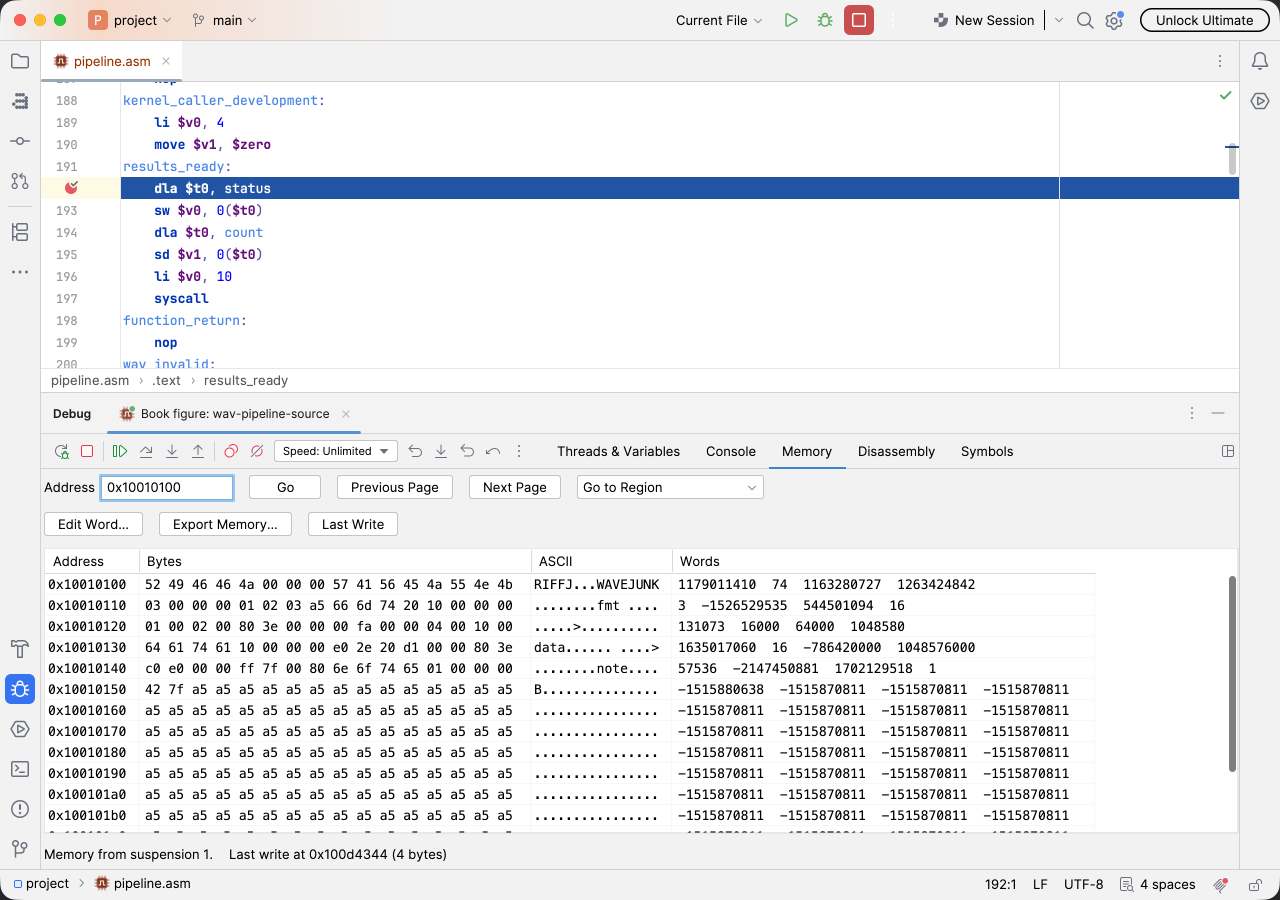
\includegraphics[width=0.84\linewidth,artifact,trim={\MARSwavpipelineinputLeft{} \MARSwavpipelineinputBottom{} \MARSwavpipelineinputRight{} \MARSwavpipelineinputTop{}},clip]{packages/031-pcm-wav/captures/f05/source.png}};
\begin{scope}[shift={(input.south west)},x={($(input.south east)-(input.south west)$)},y={($(input.north west)-(input.south west)$)}]
\draw[black,line width=0.7pt] (0.194672131,0.025641026) rectangle (0.997950820,0.833333333);
\node[draw=black,fill=white,circle,inner sep=1.5pt,font=\footnotesize] at ($(0,0.833333333)+(-3mm,0)$) {3};
\end{scope}
\node[anchor=north west,inner sep=0,font=\small\bfseries] (output-title) at ([yshift=-1mm]input.south west) {Canonical header and filtered PCM};
\node[anchor=north west,inner sep=0] (output) at ([yshift=-1mm]output-title.south west) {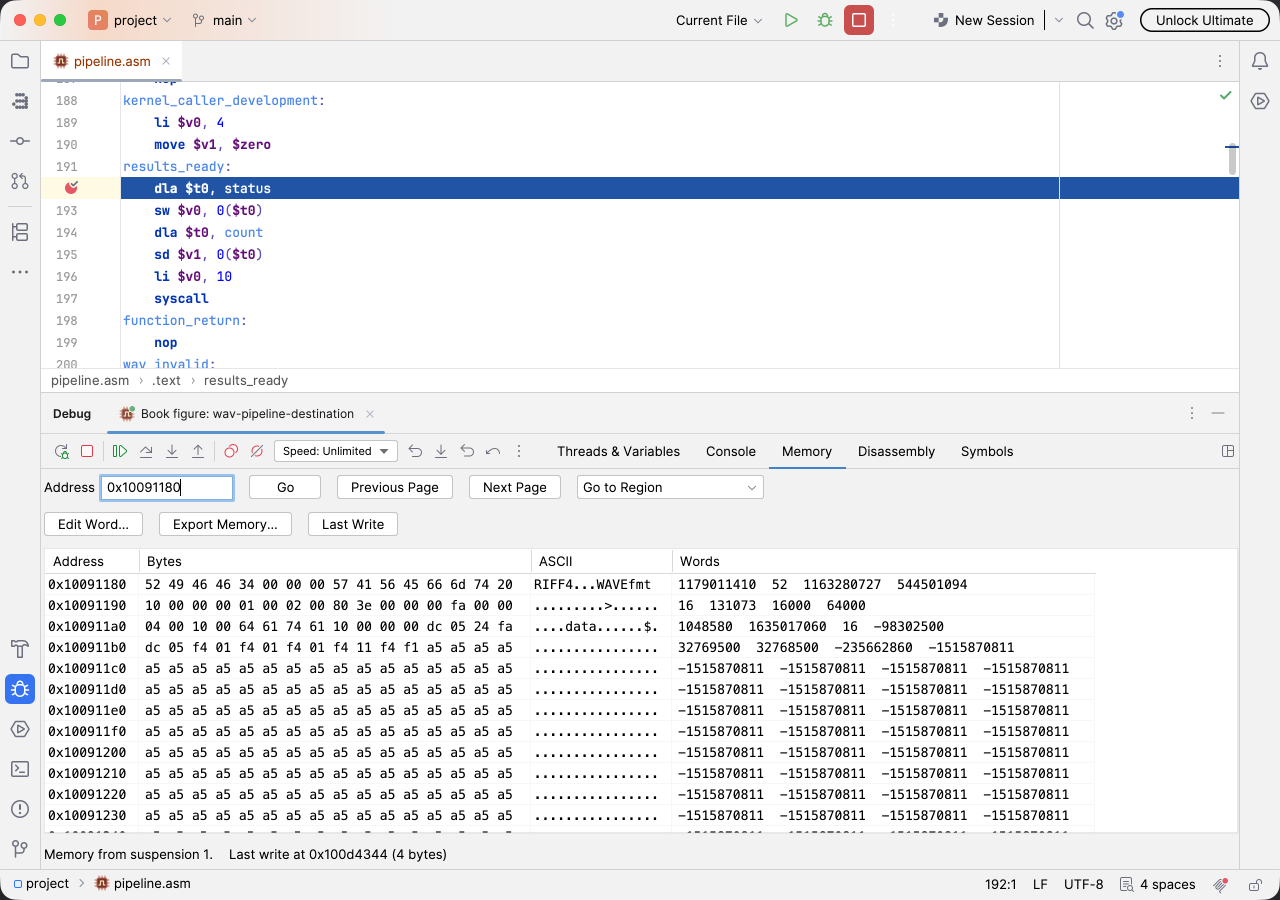
\includegraphics[width=0.84\linewidth,artifact,trim={\MARSwavpipelineoutputLeft{} \MARSwavpipelineoutputBottom{} \MARSwavpipelineoutputRight{} \MARSwavpipelineoutputTop{}},clip]{packages/031-pcm-wav/captures/f05/destination.png}};
\begin{scope}[shift={(output.south west)},x={($(output.south east)-(output.south west)$)},y={($(output.north west)-(output.south west)$)}]
\draw[black,line width=0.7pt] (0.194672131,0.035087719) rectangle (0.997950820,0.771929825);
\node[draw=black,fill=white,circle,inner sep=1.5pt,font=\footnotesize] at ($(0,0.771929825)+(-3mm,0)$) {4};
\end{scope}
\node[anchor=north west,inner sep=0,font=\small\bfseries] (clips-title) at ([yshift=-1mm]output.south west) {Separate clipped-sample count};
\node[anchor=north west,inner sep=0] (clips) at ([yshift=-1mm]clips-title.south west) {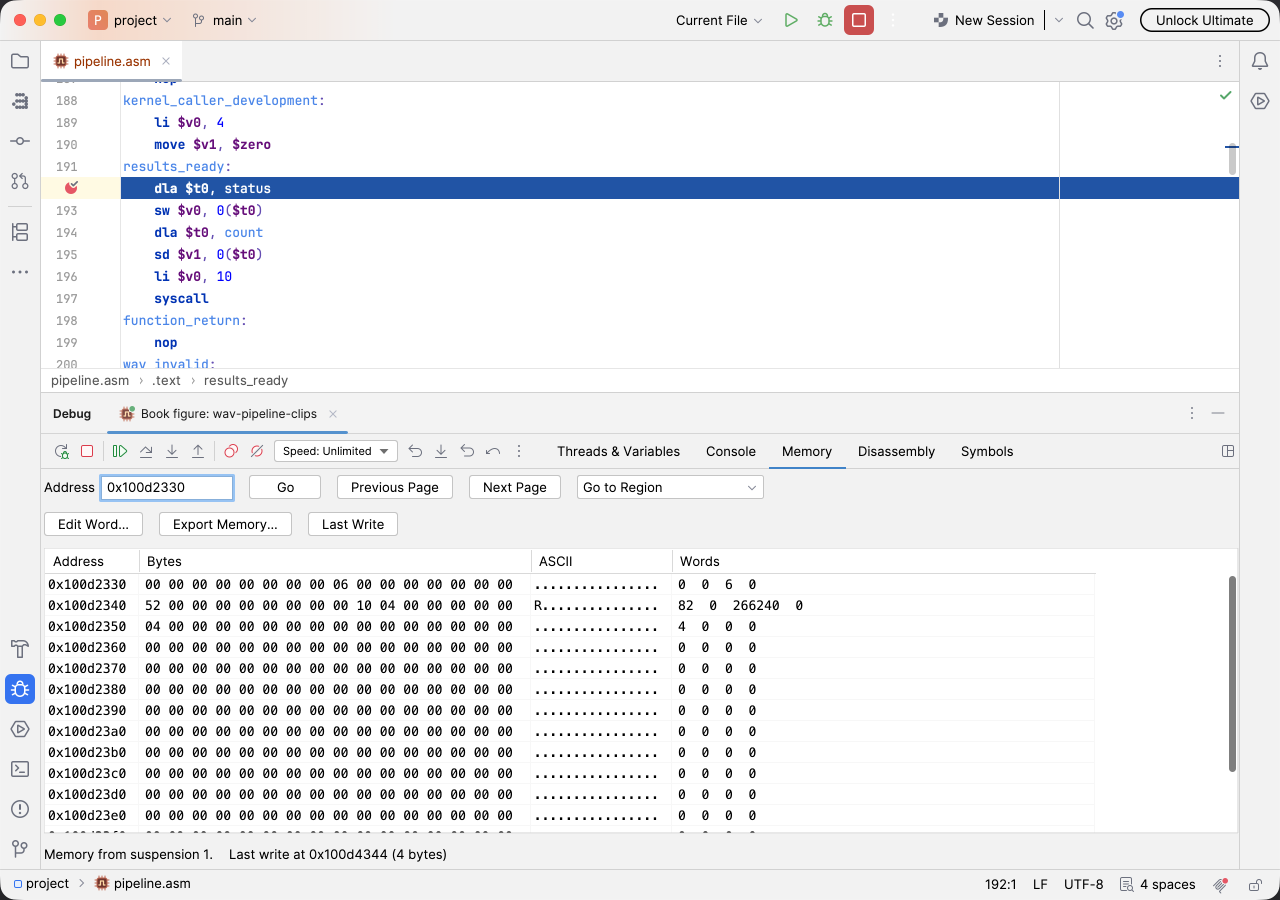
\includegraphics[width=0.84\linewidth,artifact,trim={\MARSwavpipelineclipsLeft{} \MARSwavpipelineclipsBottom{} \MARSwavpipelineclipsRight{} \MARSwavpipelineclipsTop{}},clip]{packages/031-pcm-wav/captures/f05/clips.png}};
\begin{scope}[shift={(clips.south west)},x={($(clips.south east)-(clips.south west)$)},y={($(clips.north west)-(clips.south west)$)}]
\draw[black,line width=0.7pt] (0.194672131,0.078431373) rectangle (0.997950820,0.490196078);
\node[draw=black,fill=white,circle,inner sep=1.5pt,font=\footnotesize] at ($(0,0.490196078)+(-3mm,0)$) {5};
\end{scope}
\end{tikzpicture}
\par\smallskip
\begin{minipage}{\linewidth}
\small
\begin{enumerate}
\setlength{\itemsep}{0pt}
\setlength{\parsep}{0pt}
\item At \texttt{results\_ready}, loading, parsing, filtering, encoding and saving have returned. The next instruction starts saving caller results; the file routines have already closed their descriptors.
\item \texttt{v0 = 0} reports success and \texttt{v1 = 60} is the saved output length. The returned byte length belongs to the canonical output, not the original input container.
\item The input has 82 bytes and PCM begins at offset 56. Its final \texttt{note} chunk follows the PCM. Only two bytes of the last displayed row belong to the file; later \texttt{a5} bytes are backing storage.
\item The output uses the canonical forty-four-byte header followed by sixteen filtered PCM bytes. It ends after 60 bytes; the trailing \texttt{a5} suffix is untouched. Its eight signed sample codes are 1500, $-1500$, 1500, 500, 500, 500, 4596 and $-3596$.
\item The separate eight-byte clip count is zero. The actual emitted host file is checked byte-for-byte and decoded independently. These native captures use ordinary file services; the core recipe separately verifies bounded short transfers and descriptor ownership.
\end{enumerate}
\end{minipage}
\caption{The complete pipeline turns an eighty-two-byte input into a sixty-byte canonical WAV file.}
\label{capture:031-pcm-wav-f05}
\label{pcm-wav-f05}
\end{figure}
\par
